\documentclass[10pt]{article}
\usepackage[a4paper,top=6mm,bottom=6mm,left=6mm,right=6mm,
            headheight=0pt,headsep=0pt,footskip=0pt]{geometry}
\usepackage[T1]{fontenc}
\usepackage{amsmath}
\usepackage{amssymb}
\usepackage{array}
\usepackage{xcolor}
\usepackage{tikz}
\usetikzlibrary{arrows.meta,decorations.pathreplacing}

% ================================================================
% Fractions, decimals and percentages flashcards.
%
% One card for each skill on the topic list, with a second card where
% a skill splits into different methods. Each card is written once,
% with \flashcard{<skill>}{<question>}{<answer>}, and \printflashcards
% lays them out twenty to a sheet, four across and five down: a page
% of questions followed by a page of answers.
%
% The answer page mirrors the columns, so that when the file is
% printed double-sided, flipping on the long edge, each answer lands
% on the back of its own question. The left and right margins are
% equal so that the cut lines meet on both sides of the paper. Both
% sides of a card carry its number, so a card can still be matched to
% its answer if the printer shifts the back by a millimetre or two.
%
% The answers use the wording of the Maths Revision topic list. A key
% fact from that sheet is set in bold with \key, and each card ends with
% the sheet's "Remember" line for its topic, set in bold purple with
% \remember to match the purple lines on the sheet.
%
% A card whose contents are too tall for it is drawn with a red frame
% and reported in the log as FLASHCARD OVERFLOW.
% ================================================================

\pagestyle{empty}
\setlength{\parindent}{0pt}
\setlength{\parskip}{0pt}
\setlength{\topskip}{0pt}

\newcommand{\fctopic}{Fractions, decimals and percentages}
\newcommand{\fccode}{FDP}

% ----------------------------------------------------------------
% Card layout
% ----------------------------------------------------------------
\newlength{\fcw}\setlength{\fcw}{0.25\textwidth}
\newlength{\fch}\setlength{\fch}{56mm}
\newlength{\fcpad}\setlength{\fcpad}{2mm}
\newlength{\fciw}\setlength{\fciw}{\dimexpr\fcw-2\fcpad\relax}
\newlength{\fcgap}\setlength{\fcgap}{1.2mm}
\newlength{\fcspare}
\newlength{\fcbodytop}
\newsavebox{\fcheadbox}
\newsavebox{\fcbodybox}

% \flashcard{<skill>}{<question>}{<answer>} stores one card.
\newcounter{flashcard}
\newcommand{\flashcard}[3]{%
  \stepcounter{flashcard}%
  \expandafter\gdef\csname fcskill\arabic{flashcard}\endcsname{#1}%
  \expandafter\gdef\csname fcquestion\arabic{flashcard}\endcsname{#2}%
  \expandafter\gdef\csname fcanswer\arabic{flashcard}\endcsname{#3}}

% The idea a pupil must know to answer this type of question.
\newcommand{\key}[1]{{\bfseries\boldmath #1}}
% The quick way to remember the key step, worded as on the revision sheet.
\definecolor{remember}{RGB}{112,48,160}
\newcommand{\remember}[1]{{\color{remember}\bfseries\boldmath Remember: #1}}
% A line of working, centred and in display style. Used in place of \[ \],
% which leaves an empty line above it when it follows a paragraph break.
\newcommand{\working}[1]{\par{\centering$\displaystyle #1$\par}}

\newcommand{\fcquestionstyle}{\normalsize\raggedright\setlength{\parskip}{4pt}}
\newcommand{\fcanswerstyle}{\footnotesize\raggedright\setlength{\parskip}{2pt}}

% The strip across the top of a card: the skill on the front, and the
% card number on both sides.
\newcommand{\fcnumber}[1]{\makebox[10mm][r]{\color{black!55}\fccode\ #1}}
\newcommand{\fchead}[2]{%
  \begin{minipage}{\fciw}
    \scriptsize\color{blue!50!black}%
    \if#2Q\parbox[t]{\dimexpr\fciw-10mm\relax}{\raggedright\bfseries\csname fcskill#1\endcsname}%
    \else\textbf{Answer}\fi
    \hfill\fcnumber{#1}\par
    \vspace{0.6mm}%
    {\color{blue!30}\hrule height 0.4pt}%
  \end{minipage}}

% \fccard{<number>}{Q or A} draws one side of one card. Questions sit in
% the middle of the space under the strip; answers start at the top.
\newcommand{\fccard}[2]{%
  \sbox{\fcheadbox}{\fchead{#1}{#2}}%
  \sbox{\fcbodybox}{\begin{minipage}{\fciw}%
      \if#2Q\fcquestionstyle\csname fcquestion#1\endcsname
      \else\fcanswerstyle\csname fcanswer#1\endcsname\fi
    \end{minipage}}%
  \setlength{\fcbodytop}{\dimexpr\fcpad+\ht\fcheadbox+\dp\fcheadbox+\fcgap\relax}%
  \setlength{\fcspare}{\dimexpr\fch-\fcpad-\fcbodytop-\ht\fcbodybox-\dp\fcbodybox\relax}%
  \ifdim\fcspare<0pt
    \typeout{FLASHCARD OVERFLOW: \fccode\space #1 #2 by \the\dimexpr-\fcspare\relax}%
    \def\fccut{red}%
  \else
    \typeout{FLASHCARD SPACE: \fccode\space #1 #2 has \the\fcspare\space spare}%
    \def\fccut{black!35}%
    \if#2Q\addtolength{\fcbodytop}{0.5\fcspare}\fi
  \fi
  \begin{tikzpicture}
    \useasboundingbox (0,0) rectangle (\fcw,-\fch);
    \draw[line width=0.3pt,color=\fccut] (0,0) rectangle (\fcw,-\fch);
    \node[anchor=north west,inner sep=0pt] at (\fcpad,-\fcpad) {\usebox{\fcheadbox}};
    \node[anchor=north west,inner sep=0pt] at (\fcpad,-\fcbodytop) {\usebox{\fcbodybox}};
  \end{tikzpicture}}

\newcommand{\fctitle}[2]{%
  \hbox to \textwidth{\footnotesize\vrule width 0pt height 2.6mm depth 0.9mm
    {\color{blue!50!black}\bfseries\fctopic\ flashcards}\quad
    {\color{black!60}Sheet #1 of \fcsheets: \if#2Q questions\else answers\fi}\hfil
    {\color{black!60}Print double-sided, flipping on the long edge.}}%
  \vspace{1mm}}

% \fcpage{<sheet>}{Q or A}. On the answer page the columns run right to
% left, so that each answer is printed on the back of its question.
\newcommand{\fcpage}[2]{%
  \fctitle{#1}{#2}%
  \foreach \fcrow in {1,...,5}{%
    \nointerlineskip
    \hbox{\foreach \fccol in {1,...,4}{%
      \edef\fcn{\the\numexpr(#1-1)*20+(\fcrow-1)*4+\if#2Q\fccol\else(5-\fccol)\fi\relax}%
      \ifnum\fcn>\value{flashcard}%
        \hbox to \fcw{\vrule width 0pt height \fch\hfil}%
      \else
        \fccard{\fcn}{#2}%
      \fi}}}%
  \newpage}

\newcommand{\printflashcards}{%
  \pgfmathtruncatemacro{\fcsheets}{(\the\value{flashcard}+19)/20}%
  \foreach \fcsheet in {1,...,\fcsheets}{\fcpage{\fcsheet}{Q}\fcpage{\fcsheet}{A}}}

% ----------------------------------------------------------------
% Diagrams
% ----------------------------------------------------------------
% \fracbars{<bars>}{<parts in each bar>}{<parts shaded>}{<bars in a row>}{<part width>}
% Fraction bars, each one whole, shaded in order from the first bar.
\newcommand{\fracbars}[5]{%
  \begin{tikzpicture}[x=#5,y=3mm]
    \foreach \b in {1,...,#1}{%
      \pgfmathtruncatemacro{\fcr}{(\b-1)/#4}%
      \pgfmathtruncatemacro{\fcc}{mod(\b-1,#4)}%
      \foreach \p in {1,...,#2}{%
        \pgfmathtruncatemacro{\fck}{(\b-1)*#2+\p}%
        \pgfmathsetmacro{\fcx}{\fcc*(#2+0.7)+\p-1}%
        \pgfmathsetmacro{\fcy}{-\fcr*1.5}%
        \ifnum\fck>#3\relax
          \draw (\fcx,\fcy) rectangle ++(1,1);
        \else
          \draw[fill=blue!15] (\fcx,\fcy) rectangle ++(1,1);
        \fi}}
  \end{tikzpicture}}

\begin{document}

% ================================================================
% Simplifying and ordering fractions
% ================================================================
\flashcard{Simplifying fractions}
{Write $\dfrac{36}{60}$ in its simplest form.}
{The HCF of 36 and 60 is 12, so $\div$ top and bottom by 12:
\working{\frac{36}{60}=\frac{36\div12}{60\div12}=\frac35}
Or in smaller steps:
\working{\frac{36}{60}=\frac{18}{30}=\frac9{15}=\frac35}

\remember{What you do to the numerator, do to the denominator.}}

\flashcard{Ordering fractions}
{Write these fractions in order of size, smallest first.
\working{\frac23\qquad\frac35\qquad\frac7{10}\qquad\frac56}}
{Convert to denominator 30 (the LCM of 3, 5, 10 and 6):
\working{\begin{aligned}
  \frac23&=\frac{20}{30} & \frac35&=\frac{18}{30}\\
  \frac7{10}&=\frac{21}{30} & \frac56&=\frac{25}{30}
\end{aligned}}
Smallest first: $\frac35$, $\frac23$, $\frac7{10}$, $\frac56$ (answer with the fractions as they were given)

\remember{Common denominator, then compare the numerators.}}

% ================================================================
% Mixed numbers and improper fractions
% ================================================================
\flashcard{Mixed numbers to improper fractions}
{Write $3\dfrac25$ as an improper fraction.}
{{\centering\fracbars{4}{5}{17}{2}{3.6mm}\par}
\working{3\tfrac25=\frac{3\times5+2}{5}=\frac{17}5}
(3 wholes are 15 fifths, plus 2 fifths makes 17 fifths)

\remember{Whole times denominator, add the numerator.}}

\flashcard{Improper fractions to mixed numbers}
{Write $\dfrac{23}{4}$ as a mixed number.}
{\key{Numerator $\div$ denominator: the answer gives the wholes, and the remainder stays over the denominator.}

{\centering\fracbars{6}{4}{23}{3}{2.9mm}\par}
$23\div4=5$ remainder 3, so
\working{\frac{23}4=5\tfrac34}
Check: whole times denominator, add the numerator: $5\times4+3=23$}

% ================================================================
% Adding and subtracting fractions
% ================================================================
\flashcard{Adding fractions with different denominators}
{Work out
\working{\frac34+\frac25}
Give your answer as a mixed number.}
{Common denominator 20:
\working{\begin{aligned}
  \frac34+\frac25&=\frac{15}{20}+\frac8{20}\\
                 &=\frac{23}{20}=1\tfrac3{20}
\end{aligned}}
(add the numerators; the denominator stays 20)

\remember{Common denominator. Never add the denominators!}}

\flashcard{Subtracting fractions with different denominators}
{Work out
\working{\frac56-\frac38}}
{Common denominator 24 (the LCM of 6 and 8):
\working{\frac56-\frac38=\frac{20}{24}-\frac9{24}=\frac{11}{24}}
(48 also works, but then simplify at the end)

\remember{Common denominator. Never subtract the denominators!}}

% ================================================================
% Percentages without a calculator
% ================================================================
\flashcard{Writing one number as a percentage of another}
{Amira scores 42 out of 60 in a test.

What percentage is this?}
{\working{\frac{42}{60}\times100=70\%}
Without a calculator:
\working{\frac{42}{60}=\frac7{10}=\frac{70}{100}=70\%}
(if the units are different, put both in the same units first)

\remember{Part over whole, times 100.}}

\flashcard{Finding 50\%, 10\% and 1\%}
{Without a calculator, find
\begin{tabbing}
(a) 50\% of £360\\
(b) 10\% of £360\\
(c) 1\% of £360
\end{tabbing}}
{(a) 50\%: halve.\quad $360\div2=$ £180\\
(b) 10\%: $\div10$.\quad $360\div10=$ £36\\
(c) 1\%: $\div100$.\quad $360\div100=$ £3.60

(money has two decimal places: £3.60, not £3.6)

\remember{10\%: $\div10$.\ \ 1\%: $\div100$.\ \ 50\%: halve.\ \ Then build up.}}

% ================================================================
% Converting between fractions, decimals and percentages
% ================================================================
\flashcard{Fractions to decimals and percentages}
{Write $\dfrac38$ as a decimal and as a percentage.}
{$\frac38=3\div8$, by bus stop division:

{\centering
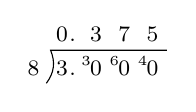
\begin{tikzpicture}[x=3.6mm,y=4.2mm,every node/.style={anchor=base,inner sep=0pt},font=\footnotesize]
  \node at (0,0) {$8$};
  \draw (0.45,-0.25) to[bend right=30] (0.6,0.75) -- (4.7,0.75);
  \node at (1,0) {$3$}; \node at (1.38,0) {.};
  \node at (2.2,0) {$0$}; \node at (3.2,0) {$0$}; \node at (4.2,0) {$0$};
  \node[font=\tiny] at (1.85,0.3) {3};
  \node[font=\tiny] at (2.85,0.3) {6};
  \node[font=\tiny] at (3.85,0.3) {4};
  \node at (1,1) {$0$}; \node at (1.38,1) {.};
  \node at (2.2,1) {$3$}; \node at (3.2,1) {$7$}; \node at (4.2,1) {$5$};
\end{tikzpicture}\par}

\working{\frac38=0.375=37.5\%}
($0.375\times100=37.5$)

\remember{Top $\div$ bottom gives the decimal; $\times100$ gives the \%.}}

\flashcard{Decimals to fractions and percentages}
{Write $0.35$ as a fraction in its simplest form, and as a percentage.}
{\key{The last digit is in the hundredths column, so the denominator is 100.}
\working{0.35=\frac{35}{100}=\frac7{20}}
($\div$ top and bottom by 5)
\working{0.35\times100=35\%}

\remember{Top $\div$ bottom gives the decimal; $\times100$ gives the \%.}}

\flashcard{Percentages to decimals and fractions}
{Write $12.5\%$ as a decimal and as a fraction in its simplest form.}
{\key{Per cent means ``out of 100'', so $\div100$ gives the decimal.}
\working{12.5\%=12.5\div100=0.125}
The last digit is in the thousandths column:
\working{0.125=\frac{125}{1000}=\frac18}
($\div$ top and bottom by 125)}

\flashcard{Ordering fractions, decimals and percentages}
{Write these numbers in order of size, smallest first.
\working{\frac23\quad\ 0.6\quad\ 65\%\quad\ \frac58\quad\ 0.67}}
{As decimals, to 3 decimal places:
\working{\begin{array}{r@{\;=\;}l@{\qquad}r@{\;=\;}l}
  \frac23 & 0.666\ldots & 0.6 & 0.600\\[3pt]
  65\%    & 0.650       & \frac58 & 0.625\\[3pt]
  0.67    & 0.670
\end{array}}
Smallest first: $0.6$, $\frac58$, $65\%$, $\frac23$, $0.67$

\remember{Turn everything into decimals, then compare them.}}

% ================================================================
% Fractions and percentages of amounts
% ================================================================
\flashcard{Fractions of amounts without a calculator}
{Without a calculator, find
\working{\frac35\text{ of }85\text{ kg}}}
{{\centering
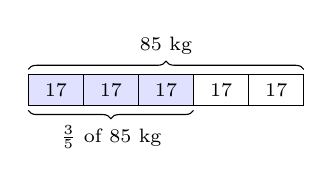
\begin{tikzpicture}[x=7mm,y=4mm,font=\scriptsize]
  \fill[blue!12] (0,0) rectangle (3,1);
  \foreach \i in {0,...,4}{\draw (\i,0) rectangle ++(1,1); \node at (\i+0.5,0.5) {17};}
  \draw[decorate,decoration={brace,amplitude=3pt}] (0,1.15) -- (5,1.15) node[midway,above=2pt] {85 kg};
  \draw[decorate,decoration={brace,amplitude=3pt,mirror}] (0,-0.15) -- (3,-0.15) node[midway,below=2pt] {$\frac35$ of 85 kg};
\end{tikzpicture}\par}

\working{85\div5=17,\quad17\times3=51}
So $\frac35$ of 85 kg is 51 kg.

\remember{Divide by the denominator, times by the numerator.}}

\flashcard{Fractions of amounts with a calculator}
{Use a calculator to find
\working{\frac7{12}\text{ of £56.40}}}
{Calculator:
\working{7\div12\times56.40=32.9}
So $\frac7{12}$ of £56.40 is £32.90 (money has two decimal places).

Check: $\frac7{12}$ is a bit more than a half, and £32.90 is a bit more than half of £56.40.

\remember{Divide by the denominator, times by the numerator.}}

\flashcard{Percentages of amounts without a calculator}
{Without a calculator, find 35\% of 260.}
{10\% of $260=26$\\
5\% $=13$ (half of 10\%)
\working{35\%=26+26+26+13=91}

\remember{10\%: $\div10$.\ \ 1\%: $\div100$.\ \ 50\%: halve.\ \ Then build up.}}

\flashcard{Percentages of amounts with a calculator}
{Use a calculator to find 17\% of £84.50.

Give your answer to the nearest penny.}
{$17\%=0.17$, so calculator:
\working{0.17\times84.50=14.365}
$=$ £14.37 to the nearest penny

Check: 10\% is about £8.50 and 20\% is about £17, so £14.37 is sensible.

\remember{Per cent means `out of 100'; `of' means multiply by.}}

% ================================================================
% Percentage change and simple interest
% ================================================================
\flashcard{Percentage change}
{The price of a bike rises from £240 to £282.

Work out the percentage increase.}
{\key{Percentage change $=\dfrac{\text{change in amount}}{\text{original amount}}\times100$}

Change $=282-240=42$
\working{\frac{42}{240}\times100=17.5\%\text{ increase}}
(divide by the original amount, not the new amount)

\remember{Change over original, times 100.}}

\flashcard{Simple interest}
{Ravi puts £400 in a savings account that pays 3\% simple interest per year.

How much is in the account after 5 years?}
{\key{Simple interest $=$ amount invested $\times$ interest rate $\times$ number of years $\div100$}

3\% of £400 $=$ £12 a year, $\times\,5=$ £60 interest

{\centering
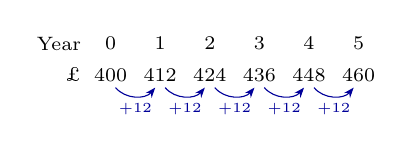
\begin{tikzpicture}[x=6.3mm,y=4mm,font=\scriptsize]
  \node[anchor=east] at (-0.4,1) {Year};
  \node[anchor=east] at (-0.4,0) {£};
  \foreach \yr/\v in {0/400,1/412,2/424,3/436,4/448,5/460}{
    \node at (\yr,1) {\yr};
    \node at (\yr,0) {\v};}
  \foreach \yr in {0,...,4}{
    \draw[-{Stealth[length=1.3mm]},blue!60!black] (\yr+0.1,-0.4) to[bend right=50] node[below=-1pt,font=\tiny] {$+12$} (\yr+0.9,-0.4);}
\end{tikzpicture}\par}

Total $=400+60=$ £460

\remember{Same interest every year: find one year, multiply by years.}}

% ================================================================
% Calculating with mixed numbers and negatives
% ================================================================
\flashcard{Adding mixed numbers}
{Work out
\working{2\frac34+1\frac23}}
{\working{\begin{aligned}
  2\tfrac34+1\tfrac23&=\frac{11}4+\frac53\\
                     &=\frac{33}{12}+\frac{20}{12}\\
                     &=\frac{53}{12}=4\tfrac5{12}
\end{aligned}}
(for adding, the wholes and the fractions can also be added separately: $3+\frac{17}{12}=4\frac5{12}$)

\remember{Mixed $\to$ improper first.}}

\flashcard{Subtracting mixed numbers}
{Work out
\working{3\frac14-1\frac23}}
{\working{\begin{aligned}
  3\tfrac14-1\tfrac23&=\frac{13}4-\frac53\\
                     &=\frac{39}{12}-\frac{20}{12}\\
                     &=\frac{19}{12}=1\tfrac7{12}
\end{aligned}}
(subtracting the wholes and the fractions separately goes wrong here, as $\frac14<\frac23$)

\remember{Mixed $\to$ improper first.}}

\flashcard{Multiplying mixed numbers}
{Work out
\working{2\frac12\times1\frac35}}
{\working{\begin{aligned}
  2\tfrac12\times1\tfrac35&=\frac52\times\frac85\\
                          &=\frac{40}{10}=4
\end{aligned}}
(multiply the tops, multiply the bottoms)

Multiplying the wholes and the fractions separately is wrong: $2\times1+\frac12\times\frac35=2\frac3{10}$, not 4.

\remember{Mixed $\to$ improper first.}}

\flashcard{Dividing mixed numbers}
{Work out
\working{3\frac13\div1\frac14}}
{\working{\begin{aligned}
  3\tfrac13\div1\tfrac14&=\frac{10}3\div\frac54\\
                        &=\frac{10}3\times\frac45\\
                        &=\frac{40}{15}=\frac83=2\tfrac23
\end{aligned}}
(keep $\frac{10}3$, change $\div$ to $\times$, flip $\frac54$ to $\frac45$)

\remember{Mixed $\to$ improper first. Dividing? Keep, change, flip. (KFC)}}

\flashcard{Fractions and negative numbers}
{Work out
\begin{tabbing}
(a)\ \ $\dfrac13-\dfrac34$\\[8pt]
(b)\ \ $-1\dfrac12\div\left(-\dfrac34\right)$
\end{tabbing}}
{(a)
\working{\frac4{12}-\frac9{12}=-\frac5{12}}
(b)
\working{\begin{aligned}
  -\frac32\div\Bigl(-\frac34\Bigr)&=-\frac32\times\Bigl(-\frac43\Bigr)\\
                                  &=\frac{12}6=2
\end{aligned}}
(negative $\times$ negative $=$ positive)

\remember{Mixed $\to$ improper first. Dividing? Keep, change, flip. (KFC)}}

\flashcard{Word problems with mixed numbers}
{A ribbon is $5\frac14$\,m long.

How many pieces $\frac34$\,m long can be cut from it?}
{How many fit into: divide.
\working{\begin{aligned}
  5\tfrac14\div\tfrac34&=\frac{21}4\div\frac34\\
                       &=\frac{21}4\times\frac43=\frac{84}{12}=7
\end{aligned}}
7 pieces

(21 quarters $\div$ 3 quarters $=7$)

\remember{Find the numbers, pick the operation, include units.}}

\flashcard{Word problems with mixed numbers}
{A rectangular rug is $2\frac12$\,m long and $1\frac13$\,m wide.

Find the area of the rug.}
{Area $=$ length $\times$ width
\working{\begin{aligned}
  2\tfrac12\times1\tfrac13&=\frac52\times\frac43\\
                          &=\frac{20}6=\frac{10}3=3\tfrac13
\end{aligned}}
Area $=3\frac13$\,m$^2$

Check: a bit more than $2\frac12\times1=2\frac12$\,m$^2$.

\remember{Find the numbers, pick the operation, include units.}}

% ================================================================
% Recurring decimals
% ================================================================
\flashcard{Recurring decimals to fractions}
{Write $0.\dot{2}\dot{7}$ as a fraction in its simplest form.}
{Let $n=0.\dot2\dot7=0.2727\ldots$\\
Two digits repeat, so $\times\,100$:
\working{\begin{array}{r@{\;}r@{\;=\;}r@{}l}
            & 100n & 27 & .2727\ldots\\
            &    n &  0 & .2727\ldots\\
  \text{subtract:} & 99n & 27 &
\end{array}}
\working{n=\frac{27}{99}=\frac3{11}}

\remember{Line up the repeats, then subtract them away. Solve algebra.}}

\flashcard{Recurring decimals to fractions}
{Write $0.1\dot{6}$ as a fraction in its simplest form.}
{Let $n=0.1\dot6=0.1666\ldots$\\
The 1 does not repeat, so use $100n$ and $10n$ to line up the repeats:
\working{\begin{array}{r@{\;}r@{\;=\;}r@{}l}
            & 100n & 16 & .6666\ldots\\
            &  10n &  1 & .6666\ldots\\
  \text{subtract:} & 90n & 15 &
\end{array}}
\working{n=\frac{15}{90}=\frac16}

\remember{Line up the repeats, then subtract them away. Solve algebra.}}

% ================================================================
% Multipliers and reverse percentages
% ================================================================
\flashcard{Percentage increase with a multiplier}
{Use a multiplier to increase £240 by 15\%.}
{\key{Multiplier for an increase $=1+\dfrac{\text{percentage}}{100}$}

{\centering
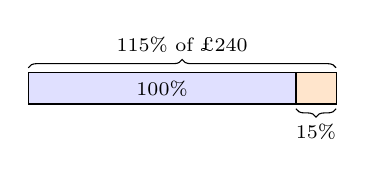
\begin{tikzpicture}[x=3.4mm,y=4mm,font=\scriptsize]
  \fill[blue!12] (0,0) rectangle (10,1);
  \fill[orange!20] (10,0) rectangle (11.5,1);
  \draw (0,0) rectangle (10,1) (10,0) rectangle (11.5,1);
  \node at (5,0.5) {100\%};
  \draw[decorate,decoration={brace,amplitude=3pt}] (0,1.15) -- (11.5,1.15) node[midway,above=2pt] {115\% of £240};
  \draw[decorate,decoration={brace,amplitude=3pt,mirror}] (10,-0.15) -- (11.5,-0.15) node[midway,below=2pt] {15\%};
\end{tikzpicture}\par}

Up 15\% $\to\times\,1.15$
\working{240\times1.15=276}
So £240 increased by 15\% is £276.

\remember{100\% plus or minus the change, then $\div100$.}}

\flashcard{Percentage decrease with a multiplier}
{A car is worth £18\,000. Its value falls by 12\%.

Use a multiplier to find its new value.}
{\key{Multiplier for a decrease $=1-\dfrac{\text{percentage}}{100}$}

{\centering
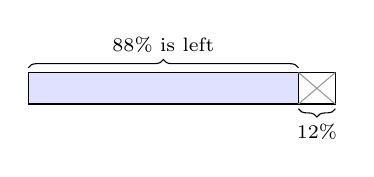
\begin{tikzpicture}[x=3.9mm,y=4mm,font=\scriptsize]
  \fill[blue!12] (0,0) rectangle (8.8,1);
  \draw (0,0) rectangle (10,1) (8.8,0) -- (8.8,1);
  \draw[black!40] (8.8,0) -- (10,1) (8.8,1) -- (10,0);
  \draw[decorate,decoration={brace,amplitude=3pt}] (0,1.15) -- (8.8,1.15) node[midway,above=2pt] {88\% is left};
  \draw[decorate,decoration={brace,amplitude=3pt,mirror}] (8.8,-0.15) -- (10,-0.15) node[midway,below=2pt] {12\%};
\end{tikzpicture}\par}

Down 12\% $\to\times\,0.88$
\working{18\,000\times0.88=15\,840}
The new value is £15\,840.

\remember{100\% plus or minus the change, then $\div100$.}}

\flashcard{Finding the original amount}
{In a sale, everything is 20\% off. A coat costs £64 in the sale.

What was the original price of the coat?}
{\key{Original amount $=$ new amount $\div$ multiplier}

{\centering
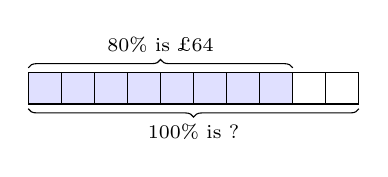
\begin{tikzpicture}[x=4.2mm,y=4mm,font=\scriptsize]
  \fill[blue!12] (0,0) rectangle (8,1);
  \foreach \i in {0,...,9}{\draw (\i,0) rectangle ++(1,1);}
  \draw[decorate,decoration={brace,amplitude=3pt}] (0,1.15) -- (8,1.15) node[midway,above=2pt] {80\% is £64};
  \draw[decorate,decoration={brace,amplitude=3pt,mirror}] (0,-0.15) -- (10,-0.15) node[midway,below=2pt] {100\% is ?};
\end{tikzpicture}\par}

20\% off $\to\times\,0.8$: $0.8\times\text{original}=64$
\working{\text{original}=64\div0.8=\text{£}80}
Check: 10\% is £8, 100\% is £80.

\remember{Going backwards? Divide by the multiplier!}}

\flashcard{Finding the original amount}
{After a 20\% pay rise, Jo earns £360 a week.

How much did Jo earn each week before the pay rise?}
{\key{Original amount $=$ new amount $\div$ multiplier}

{\centering
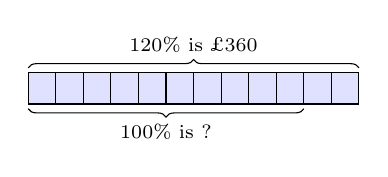
\begin{tikzpicture}[x=3.5mm,y=4mm,font=\scriptsize]
  \fill[blue!12] (0,0) rectangle (12,1);
  \foreach \i in {0,...,11}{\draw (\i,0) rectangle ++(1,1);}
  \draw[decorate,decoration={brace,amplitude=3pt}] (0,1.15) -- (12,1.15) node[midway,above=2pt] {120\% is £360};
  \draw[decorate,decoration={brace,amplitude=3pt,mirror}] (0,-0.15) -- (10,-0.15) node[midway,below=2pt] {100\% is ?};
\end{tikzpicture}\par}

Up 20\% $\to\times\,1.2$: $1.2\times\text{original}=360$
\working{\text{original}=360\div1.2=\text{£}300}
Check: 10\% is £30, 100\% is £300.

\remember{Going backwards? Divide by the multiplier!}}

\printflashcards

\end{document}
